\usetikzlibrary{patterns}

\newcommand{\animateCell}[2]{   % x,y
    \begin{textblock}{\boardSize}[0,0](0,0)
        \begin{animateinline}[nomouse,label={cell#1x#2}]{1}
            \drawCell{#1}{#2}{0}  \newframe % empty
            \drawCell{#1}{#2}{1}  \newframe % tail pointing down
            \drawCell{#1}{#2}{2}  \newframe % tail pointing right
            \drawCell{#1}{#2}{3}  \newframe % tail pointing up
            \drawCell{#1}{#2}{4}  \newframe % tail pointing left
            \drawCell{#1}{#2}{5}  \newframe % face pointing up
            \drawCell{#1}{#2}{6}  \newframe % face pointing left
            \drawCell{#1}{#2}{7}  \newframe % face pointing down
            \drawCell{#1}{#2}{8}  \newframe % face pointing right
            \drawCell{#1}{#2}{9}  \newframe % dead face pointing up
            \drawCell{#1}{#2}{10} \newframe % dead face pointing left
            \drawCell{#1}{#2}{11} \newframe % dead face pointing down
            \drawCell{#1}{#2}{12} \newframe % dead face pointing right
            \drawCell{#1}{#2}{13} \newframe % straight horizontal
            \drawCell{#1}{#2}{14} \newframe % straight vertical
            \drawCell{#1}{#2}{15} \newframe % angle up right
            \drawCell{#1}{#2}{16} \newframe % angle up left
            \drawCell{#1}{#2}{17} \newframe % angle down left
            \drawCell{#1}{#2}{18} \newframe % angle down right
            \drawCell{#1}{#2}{19}           % food
        \end{animateinline}
    \end{textblock}
}

\newcommand{\drawHappyFace}{
    \draw[fill=green!50!white] (0.5,0.5) circle (0.3);
    \path[fill=black,draw=white,thick] (0.4,0.6) circle (0.03) (0.6,0.6) circle (0.03);
    \draw[fill=orange] (0.5,0.48) circle (0.03);
    \draw (0.5,0.48) ++(-160:0.15) arc (-160:-20:0.15);
}
\newcommand{\drawSadFace}{
    \draw[fill=red!50!white] (0.5,0.5) circle (0.3);
    \path[fill=black,draw=white,thick] (0.4,0.6) circle (0.03) (0.6,0.6) circle (0.03);
    \draw (0.5,0.44) ++(-160:0.15) arc (160:20:0.15);
}

\newcommand{\drawStraightSegment}[1]{
    \begin{scope}[rotate around={#1:(0.5,0.5)}]
        \path[fill=green!40!blue] (0,0.15) -- (1,0.15) -- (1,0.85) -- (0,0.85);
        \path[draw] (0,0.15) -- (1,0.15) (1,0.85) -- (0,0.85);
    \end{scope}
}

\newcommand{\drawEndSegment}[1]{
    \begin{scope}[rotate around={#1:(0.5,0.5)}]
        \path[fill=green!40!blue] (0.15,0) -- (0.15,0.5) arc (180:0:0.35)  -- (0.85,0);
        \path[draw] (0.15,0) -- (0.15,0.5) arc (180:0:0.35)  -- (0.85,0);
    \end{scope}
}

\newcommand{\drawAngleSegment}[1]{
    \begin{scope}[rotate around={#1:(0.5,0.5)}]
        \path[fill=green!40!blue] (1,0.15){[rounded corners=0.35cm] -- (0.15,0.15)} -- (0.15,1) -- (0.85,1) {[rounded corners=0.1cm] -- (0.85,0.85)} -- (1,0.85);
        \path[draw] (1,0.15){[rounded corners=0.35cm] -- (0.15,0.15)} -- (0.15,1) (0.85,1) {[rounded corners=0.1cm] -- (0.85,0.85)} -- (1,0.85);
    \end{scope}
}

\newcommand{\drawFood}{
    \draw[fill=brown!70!white] (0.5,0.43) ellipse (0.31 and 0.15);
    \draw[fill=blue!80!white] (0.2,0.4) -- (0.3,0.1) -- (0.7,0.1) -- (0.8,0.4) to[out=-150,in=-30] (0.2,0.4);
    \draw (0.4,0.1) -- (0.35,0.33) (0.5,0.1) -- (0.5,0.31) (0.6,0.1) -- (0.65,0.33);
    \draw[fill=red!50!white] (0.5,0.55) ellipse (0.2 and 0.05);
    \draw[fill=orange!50!yellow] (0.5,0.8) -- (0.46,0.84) arc (200:160:0.08) -- (0.5,0.98) -- (0.54,0.89) arc (20:-20:0.08) -- cycle;
    \draw[fill=white] (0.47,0.57) rectangle (0.53,0.8);
    \draw[pattern=north east lines,pattern color=red] (0.47,0.57) rectangle (0.53,0.8);
}

\newcommand{\drawSnakeSegment}[1]{
    \ifthenelse{#1=1}{ \drawEndSegment{180}}{}
    \ifthenelse{#1=2}{ \drawEndSegment{270}}{}
    \ifthenelse{#1=3}{ \drawEndSegment{0}  }{}
    \ifthenelse{#1=4}{ \drawEndSegment{90} }{}
    \ifthenelse{#1=5}{ \drawEndSegment{0}   \drawHappyFace}{}
    \ifthenelse{#1=6}{ \drawEndSegment{90}  \drawHappyFace}{}
    \ifthenelse{#1=7}{ \drawEndSegment{180} \drawHappyFace}{}
    \ifthenelse{#1=8}{ \drawEndSegment{270} \drawHappyFace}{}
    \ifthenelse{#1=9}{ \drawEndSegment{0}   \drawSadFace}{}
    \ifthenelse{#1=10}{\drawEndSegment{90}  \drawSadFace}{}
    \ifthenelse{#1=11}{\drawEndSegment{180} \drawSadFace}{}
    \ifthenelse{#1=12}{\drawEndSegment{270} \drawSadFace}{}
    \ifthenelse{#1=13}{\drawStraightSegment{0} }{}
    \ifthenelse{#1=14}{\drawStraightSegment{90}}{}
    \ifthenelse{#1=15}{\drawAngleSegment{0}  }{}
    \ifthenelse{#1=16}{\drawAngleSegment{90} }{}
    \ifthenelse{#1=17}{\drawAngleSegment{180}}{}
    \ifthenelse{#1=18}{\drawAngleSegment{270}}{}
    \ifthenelse{#1=19}{\drawFood}{}
}

\newcommand{\drawCell}[3]{  % x,y,segment
    \begin{tikzpicture}
        \path[use as bounding box,draw] (0,0) rectangle (\gameSize,\gameSize);
        \begin{scope}[shift={(#1,#2)}]
            \drawSnakeSegment{#3}
        \end{scope}
    \end{tikzpicture}
}

\newcommand{\drawBackground}{
    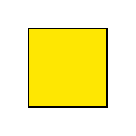
\begin{tikzpicture}
        \path[use as bounding box,draw] (0,0) rectangle (\gameSize,\gameSize);
        \draw[fill=yellow!90!orange] (0,0) rectangle (\gameSize,\gameSize);
    \end{tikzpicture}
}

\newcommand{\drawIntro}{
    \begin{tikzpicture}
        \path[fill=yellow!90!orange,use as bounding box] (0,0) rectangle (\gameSize,\gameSize);
        \begin{scope}[shift={(\gameSize/2,\gameSize/2)}]
            \draw[rounded corners=0.5cm,fill=white] (-3,-3) rectangle (3,3);
            \node at (0,2) {\large \textbf{teXnake}};
            \draw[rounded corners=0.1cm] (-2,0.5) rectangle (-0.3,1) ++ (-0.85,-0.25) node {Space};
            \draw[rounded corners=0.1cm] (-2,-1.35) rectangle ++(0.5,0.5) ++ (-0.25,-0.25) node {A};
            \draw[rounded corners=0.1cm] (-1.4,-1.35) rectangle ++(0.5,0.5) ++ (-0.25,-0.25) node {S};
            \draw[rounded corners=0.1cm] (-0.8,-1.35) rectangle ++(0.5,0.5) ++ (-0.25,-0.25) node {D};
            \draw[rounded corners=0.1cm] (-1.4,-0.75) rectangle ++(0.5,0.5) ++ (-0.25,-0.25) node {W};
            \node at (1.3,0.75) {Start game};
            \node at (1.3,-0.8) {Move};
            \node at (0,-2.2) {Adobe Reader is required to play};
        \end{scope} 
    \end{tikzpicture}
}